\documentclass[11pt]{article}
\usepackage{fullpage}
\usepackage{fancyhdr}
\usepackage{epsfig}
\usepackage{multienum}
\usepackage{algorithm}
\usepackage[noend]{algorithmic}
\usepackage{amsmath,amssymb,amsthm}
\usepackage{ifsym}
\usepackage{graphicx}
\usepackage{cite}

\usepackage{xcolor}
\usepackage{listings}
\usepackage{minted}
\usemintedstyle{vs}
\usepackage{xparse}

\newtheorem{lemma}{Lemma}
\newtheorem*{lem}{Lemma}
\newtheorem{definition}{Definition}
\newtheorem*{definition*}{Definition}
\newtheorem{notation}{Notation}
\newtheorem*{claim}{Claim}
\newtheorem*{fclaim}{False Claim}
\newtheorem{observation}{Observation}
\newtheorem{conjecture}[lemma]{Conjecture}
\newtheorem{theorem}[lemma]{Theorem}
\newtheorem{corollary}[lemma]{Corollary}
\newtheorem{proposition}[lemma]{Proposition}
\newtheorem*{rt}{Running Time}

\def\P{\ensuremath{\mathcal{P}}}
\def\s{\ensuremath{{\bf s}}}
\def\p{\ensuremath{{\bf p}}}
\def\opt{\ensuremath{\textsc{opt}}}

\textheight=8.6in
\setlength{\textwidth}{6.44in}
\addtolength{\headheight}{\baselineskip} 
% enumerate uses a., b., c., ...
\renewcommand{\labelenumi}{\bf \alph{enumi}.}
% Sets the style for fancy pages (namely, all but first page)
\pagestyle{fancy}
\fancyhf{}
\renewcommand{\headrulewidth}{0.0pt}
\renewcommand{\footrulewidth}{0.4pt}
% Changes style of plain pages (namely, the first page)
\fancypagestyle{plain}{
  \fancyhf{}
  \renewcommand\headrulewidth{0pt}
  \renewcommand\footrulewidth{0.4pt}
  \renewcommand{\headrule}{}
}

\title{Screeps Lite: An Environment of Exploration, Emergence, Greediness, and Sabotage}
\author{Eren Guendelsberger, Jake Israel, and James Capuder}
\date{Spring 2017}

\NewDocumentCommand{\codeword}{v}{%
\texttt{\textcolor{blue}{#1}}%
}

\lstset{language=Python,keywordstyle={\bfseries \color{blue}}}


\begin{document}
\maketitle
\thispagestyle{plain}

\begin{abstract}
Q-Learning, and the numerous extensions thereof, has become a ubiquitous reinforcement learning technique. To explore the effectiveness of Q-Learning in training multiple agents to farm resources, a training environment was implemented Python (3.5). The modular nature of the developed environment allowed for the simulation of various scenarios and reward structures, and for the possibility of future extensions.
\end{abstract}

\section{Introduction}

	The primary goal of this project was to explore the phenomenon of emerging intelligence in multi-agent systems. Using an environment containing multiple non-communicating agents allowed for the observation of the strategies they developed to maximize individual utility. By testing different environments and different types of agents, global patterns of cooperation and competition emerged. 
	
	Initially, Screeps seemed like a good environment to perform these experiments in. Once we tried to implement Q-learning however, several problems emerged. Because the Screeps world has a fixed amount of time between steps and it is very difficult to save and restore specific board states, it would have taken far too long for any meaningful learning to occur. In addition, the state space is so large that any single state would likely have never been encountered again. Finally, many of the interesting problems such as pathfinding were already solved. 
	
	Because of this, it made the most sense to do this project in a simplified Screeps-like environment without the limitations of a preexisting online game. The goal of a standard agent is to gather resources from a source and bring them back to a spawn. In later environments we narrowed the focus of each agent, dividing them up into gatherers, carriers, and thieves. This allowed us to observe how the agents would act when they were forced to work together and how they would handle threats. By creating this simple clone of Screeps, we obtained more direct control over our experiments. The ability to reload and modify the starting environment and do thousands of episodes of learning in a very short time allowed for the unobstructed observation of the performance of learning methods in a multiagent system. 
	
\section{Prior Research}

As discussed above, one shortcoming of \textit{Screeps} for this project was the lack of any prior Artificial Intelligence research related to the game (perhaps foreshadowing the conclusions that lead to our shift in focus). Reinforcement Learning as a technique for building bots to play games, however, is a common research subject. Though our environment and learning methods were relatively simple, resources providing background on Reinforcement Learning offered valuable supplemental information to that covered in lecture.

\section{Implementation}

This section details the implementation of the scripts and classes used in our framework: \textit{tile.py, state.py, source.py, spawn.py, agent.py, grid.py, environment.py,} and finally \textit{qlearning.py}.

\subsection{Tile}

The class used to represent each square on the grid in our simulation is \codeword{Tile}. The constructor, \mintinline{Python}{def __init__(self, x, y, tile_type)}, takes as arguments the $x$ and $y$ positions of the \codeword{Tile} on the grid, and a character representing what type of tile to initialize. These are saved as instance variables; $x, y$ are static, but \mintinline{Python}{tile_type} along with a variable \mintinline{Python}{self.init_type} to save the initial type of the tile so that the grid can be reset to it's initial configuration. The following table contains the mapping of characters to the tile types the represent.

\begin{table}[h]
\centering
\caption{Character to type mapping}
%\label{my-label}
\begin{tabular}{|l|l|}
\hline
Character & Type \\ \hline
o & Empty \\ \hline
s & Spawn \\ \hline
r & Source \\ \hline
a & Agent \\ \hline
x & Obstacle \\ \hline
g & Gatherer \\ \hline
c & Carrier \\ \hline
t & Thief \\ \hline
\end{tabular}
\end{table}

Additionally, each \codeword{Tile} instance keeps track of adjacent tiles to the north, east, south, and west of the instance in a dictionary. This dictionary cannot be constructed until all tiles are initialized, so the method to do so, \mintinline{Python}{initAdjacent(self, grid)}, is not called on instance initialization.

\subsection{State}

The class \codeword{State} simply holds constants that are used to clarify the indexing of the three-tuple representing each \codeword{Agent}'s state, which is discussed below.

\subsection{Source}

A source\footnote{refered to as such in the code, but as a resource in the following results section} is an object from which agents can collect energy to return to the spawn. The constructor, \mintinline{Python}{__init__(self, x, y, capacity=100000)}, takes $xy$ coordinates and a capacity, which is the maximum amount that can be farmed from the source. The \mintinline{Python}{gather(self)} method is called whenever an agent gathers from this source, and returns a boolean value indicating whether the action was successful (false if \mintinline{Python}{self.capacity==0}, true otherwise). Similarly to \codeword{Tile}, \codeword{Source} has a reset method that reverts \mintinline{Python}{self.capacity} to the value with which it was initialized.

\subsection{Spawn}

\codeword{Spawn} objects are those to which agents return gathered resources. The constructor, \mintinline{Python}{__init__(self, x,y)}, takes only the $xy$ position of the \codeword{Spawn} instance on the grid. The \mintinline{Python}{dropoff(self)} method increments a counter representing the total number of resources returned to this \codeword{Spawn} whenever an agent performs that action, and the reset method reverts that counter to 0.

\subsection{Agent}

\codeword{Agent} is a more substantial class than those previously discussed. The constructor, \mintinline{Python}{__init__(self,environment, x, y, carry, agent_type)}, accepts an environment object, the starting $xy$ position on the grid, a boolean \mintinline{Python}{carry}, and the type of agent to be initialized. The agent's initial state is then constructed as the three-tuple of \mintinline{Python}{(x, y, carry)}. Instance variables include the agent's Q-table as a dictionary, cumulative reward, capacity (number of resources the agent can carry, always 1), a boolean representing whether the agent's reward should be reduced (for use in the prisoner's dilemma scenario), two initially null variables indicating the agent's victim (for the thief scenario), and the agent to hand resources to (in the collaborative scenario).

\codeword{Agent} has methods:
\begin{itemize}
\item \mintinline{Python}{update_position(self, x, y)}, which changes the coordinates in the instance's state;
\item \mintinline{Python}{do_action(self, action, alpha, discount_factor, reward_modifier)} simulates an agent picking an action, calculating the reward, updating the Q-table, and returning the reward;
\item \mintinline{Python}{mock_action(self, action)}, which makes use of the environment's mock action method to return the reward for an action without actually updating the Q-table or the agent's state;
\item \mintinline{Python}{get_q(self, state, action)} which extracts an entry from the the Q-table, or 0 if no entry exists;
\item \mintinline{Python}{update_q(self, state, action, reward, alpha, discount_factor)}, which is called by \mintinline{Python}{do_action(...)} to perform the calculations on the inputs needed to update the Q-table;
\item \mintinline{Python}{get_explorative_action(self)} which returns a random action from the set of possible actions;
\item \mintinline{Python}{get_exploitative_action(self)}, which returns the action with the highest Q given the agent's current state;
\item \mintinline{Python}{pick_action_epsilon(self, epsilon)}, which selects an action by the epsilon greedy approach;
\item \mintinline{Python}{pick_action_softmax(self, tau)}, which selects an action by the softmax approach;
\item \mintinline{Python}{get_actions(self)}, which calls the environment's \mintinline{Python}{get_agent_actions()} method to get the available actions to this agent;
\item and finally \mintinline{Python}{reset(self)} to revert to the original state and reset the cumulative reward to 0.
\end{itemize}


\subsection{Grid}

\codeword{Grid} is a relatively simple class responsible for building and managing a board of tile objects.The constructor for \codeword{Grid}, \mintinline{Python}{__init__(self, fpath, environment)}, takes an environment object and a file path pointing to a text file containing an initial board configuration. It initializes lists of agents, spawns, and sources, splits the contents of the text file into a 2D list, infers \mintinline{Python}{self.width, self.height} from that list, and finally builds up the actual board by reading each character in the 2D list, and constructing a new \codeword{Tile} object for each one with the appropriate type and $xy$ position.

\codeword{Grid} implements the following methods:

\begin{itemize}
\item \mintinline{Python}{initTileAdjacent(self)}, which is called after \mintinline{Python}{self.board} is constructed. This method populates the lists \mintinline{Python}{self.agents, self.spawns, self.sources}, and calls each tile's \mintinline{Python}{initAdjacent()} method.
\item \mintinline{Python}{get_tile(self, x, y)} returns the tile at \mintinline{Python}{self.board[y][x]}.
\item \mintinline{Python}{reset(self)} which calls the appropriate reset method on all elements of the three lists discussed above, as well as the reset method of each tile.
\item \mintinline{Python}{reset_all(self, components)} which simply takes a list of elements and calls that element's reset method.
\end{itemize}

\subsection{Environment}

Now that we have the various components of our simulation, we cover the \codeword{Environment} class, which effectively serves as the shared point between \codeword{Grid} and \codeword{Agent}, helping to define how the agents are allowed to move around the grid. The constructor for \codeword{Environment}, \mintinline{Python}{__init__(self, fname)}, takes just a file name, which is used to initialize a \codeword{Grid} instance. An important note is that the constructors for both \codeword{Grid} and \codeword{Agent} both take an environment object, so the environment from which this \codeword{Grid} is created, is propagated to all of these objects. The only instance variables of \codeword{Environment} are the \codeword{Grid} and a boolean value indicating whether the current episode is finished.

\codeword{Environment} contains the following methods:

\begin{itemize}
\item \mintinline{Python}{get_all_agents(self)}, which returns the list of agents stored in \mintinline{Python}{self.grid}
\item \mintinline{Python}{get_agent_actions(self, agent)}, which takes an agent and returns a list of legal moves the agent can take. This list is constructed by a series of boolean checks on the type of tile the agent is on and the agent's state, and can modify the agent's \mintinline{Python}{victim} and \mintinline{Python}{handoffee} variables when appropriate.
\item \mintinline{Python}{get_agent_on_tile(self, tile)} returns the agent on the specified tile, if one exists. This is used by \mintinline{Python}{get_agent_actions(...)} when interaction between agents is allowed.
\item \mintinline{Python}{adjacent_resource(self, agent)} returns a tile adjacent to \mintinline{Python}{agent} that has a source, or simply \mintinline{Python}{agent}'s current tile if no adjacent source exists.
\item \mintinline{Python}{do_action(self,agent,action)} takes an agent and an action, and returns the reward for that action. The difference between this and \mintinline{Python}{Agent.do_action(...)} is that this method performs the state changes on agents, the modification of the board, and the setting of instance variables only, and relies on the \mintinline{Python}{agent} to perform all additional calculations to transform the raw value of the reward returned here into what actually ends up in the \mintinline{Python}{agent}'s Q-table.
\end{itemize}

  
\subsection{Qlearning}

This is the script that actually runs the episodes, plots the data, and manages the basic GUI (enabled by setting the gui_enabled boolean to True). \mintinline{Python}{ENV_FILE} is set to the name of a text file containing the initial configurations for a scenario, only one of which can be uncommented at a time. \mintinline{Python}{NUM_EPISODES, NUM_STEPS} define the number of episodes to run for each Q-learning method, and the number of steps per episode, respectively. \mintinline{Python}{EPSILON_MODE, EPSILON1, EPSILON2} are, in order: a 0 or 1, representing whether the epsilon greedy approach should be performed, the first value for epsilon to use for simulation, and the second epsilon value to use for simulation. \mintinline{Python}{SOFTMAX_MODE} determines whether the softmax approach should be performed, and \mintinline{Python}{TAU} specifies the tau value for use in softmax.

The main method calls \mintinline{Python}{qlearning(environment, num_episodes, discount_factor, mode, epsilon=0)} for each enabled learning mode, parameterized by the flags set at the beginning of the script. This method in turn runs each episode by calling \mintinline{Python}{qlearn_episode(agents,discount_factor, mode, epsilon, episode)}, which returns a list of the cumulative rewards earned by each agent to \mintinline{Python}{qlearning(...)}. Each episode's results are saved in a list that is returned to main, and the information is then plotted with \mintinline{Python}{matplotlib}.  


\section{Results}

We tested our multi-agent q-learning implementation on a number of Screeps-like environments. We found some interesting and emergent results.

\subsection{A Better Reward Lies Farther Away}

For the first environment, we started the agent near a resource that was far away from a spawn. Way down south, there was another resource and spawn pair very close to each other. The map looks as follows.\\
\texttt{
soooaooor\\
ooooooooo\\
ooxoooooo\\
ooooooooo\\
ooooooooo\\
ooooooooo\\
ooooooooo\\
oooooosor\\
}
"o" means empty tile, "s" means spawn, "r" means resource, "a" means agent starting point, and "x" means blockade. We get the following results for the agent when running it for 1000 episodes in this environment.\\

\begin{figure}[h]
  \centering
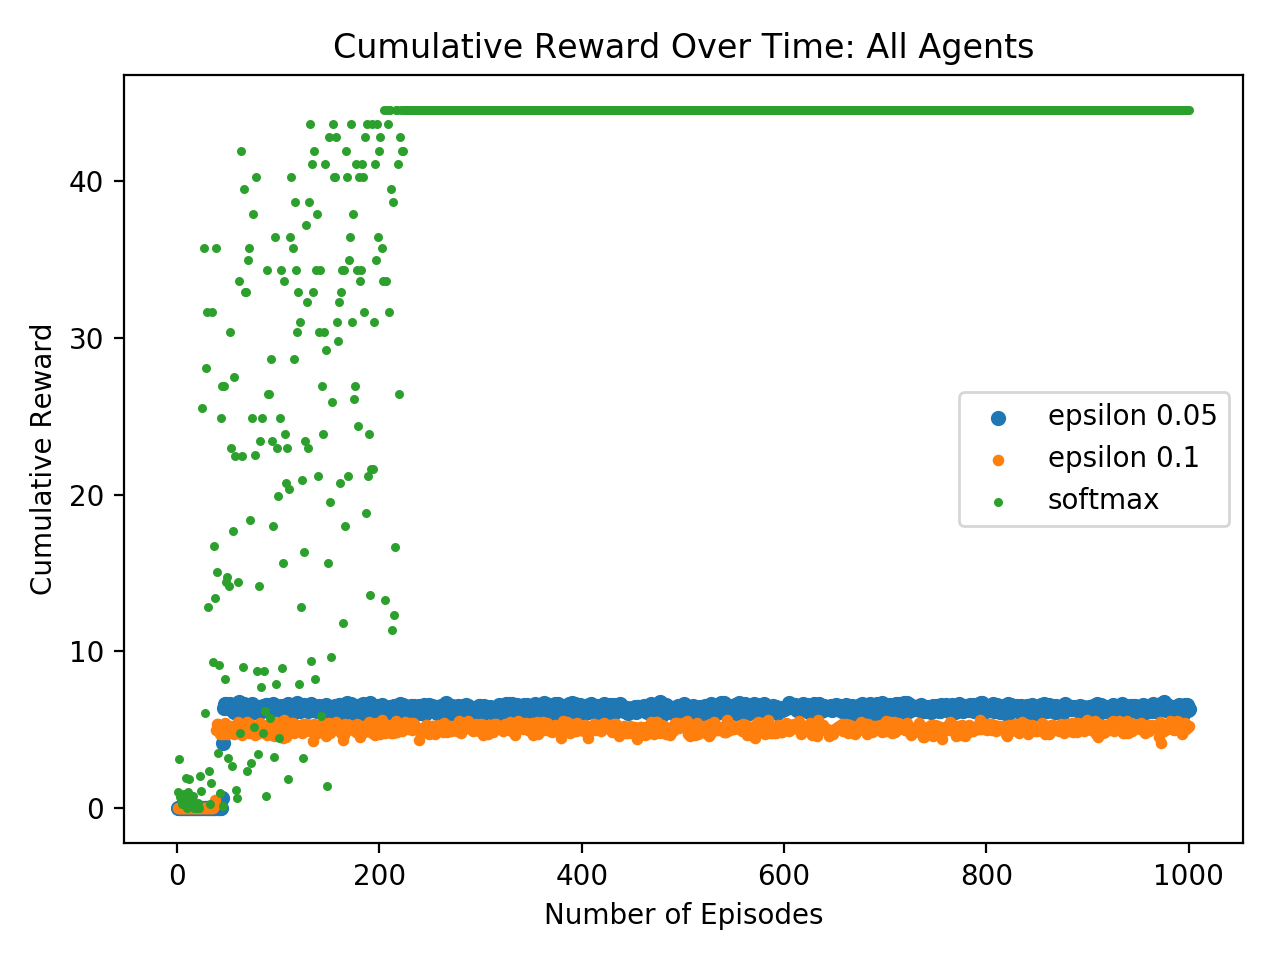
\includegraphics[width=.7\textwidth]{ai-env1.png}
\caption{Single agent cumulative reward, 1000 episodes.}
\end{figure}
%[insert ai-env1.png]\\

We notice that the two epsilon-greedy action selectors perform similarly, with a slight preference to an epsilon of 0.05. Once they find the nearby resource and spawn and learn what to do, they immediately jump up significantly in reward, thanks to the lack of unpredictable results with the actions. However, they never find the farther away resource that has a close spawn. Since they only explore less than 10\% of the time, they never stray far enough away from the initial reward sequence they find to get to the other one. The variance is quite low for both of the epsilon-greedy algorithms. The little variance we notice after the improvement is due to the exploration. As we would expect, the results with an epsilon of 0.05 has less variance than the results with an epsilon of 0.1.

On the other hand, the softmax algorithm finds the better reward. The frequency of exploration for softmax depends on how well the algorithm is currently doing, that is to say based on how high the Q-values are. When the Q-values for the exploitative actions eclipses those of the other possible actions, the algorithm will rarely pick non-exploratory actions. The softmax algorithm is not satisfied by the resource, spawn pair that are far apart, as the q-values do not get high enough to significantly reduce exploration. This causes a significant amount of variance at the beginning of the episode. Eventually, the algorithm finds the close resource, spawn pair and learns to go there immediately at the start of the episode. Since it receives a reward every other turn (as they are right next to each other) it is very unlikely for it to explore. As a result, the variance is almost zero once the algorithm converges. As it is learning, however, the variance is significantly higher than the maximum variance interval of either of the epsilon-greedy algorithms.

\subsection{A Dilemma}

For this environment, we have two agents. The first agent starts near the far away resource, spawn pair, and the second agent starts next to the close resource, spawn pair. Note that if multiple agents mine the same resource simultaneously, they both get less than 50\% of what they would otherwise due to overcrowding.\\
\texttt{
soooaooor\\
ooooooooo\\
ooxoooooo\\
ooooooooo\\
ooooooooo\\
oooooooos\\
ooooooooa\\
oooooosor\\
}

We generated graphs for each agent individually and for the environment as a whole. The purpose of this was to analyze whether greedy behavior hurts overall utility, and it does. We first present Agent 1's graph, the agent who started near the far away source, resource pair.

%[insert ai-env2-agent1.png]\\

\begin{figure}[h]
  \centering
  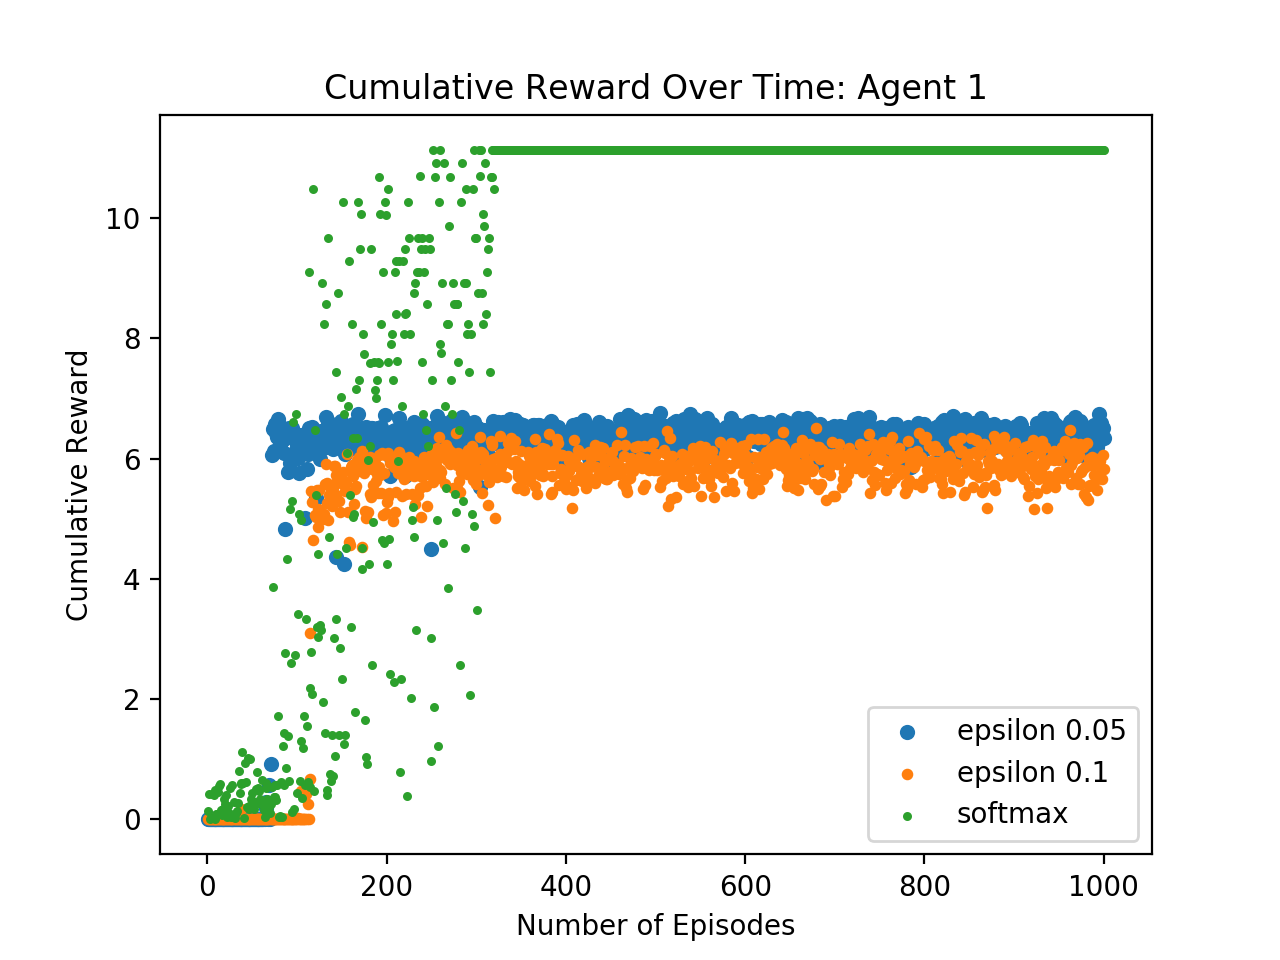
\includegraphics[width=.7\textwidth]{ai-env2-agent1.png}
  %\caption{Environment 2, agent 1 cumulative reward}
\end{figure}

For the epsilon algorithms, agent 1 again never finds the closer resource, spawn pair, and its performance is mediocre. However, this also means that it does not hurt the other agent. The softmax algorithm is again able to find the closer pair. This time, the agent does not gain as much reward as before due to overcrowding, but it still gains more than when it was at the farther away resource. We now analyze agent 2 individually.
%[insert ai-env2-agent2.png]\\

\begin{figure}[h]
  \centering
  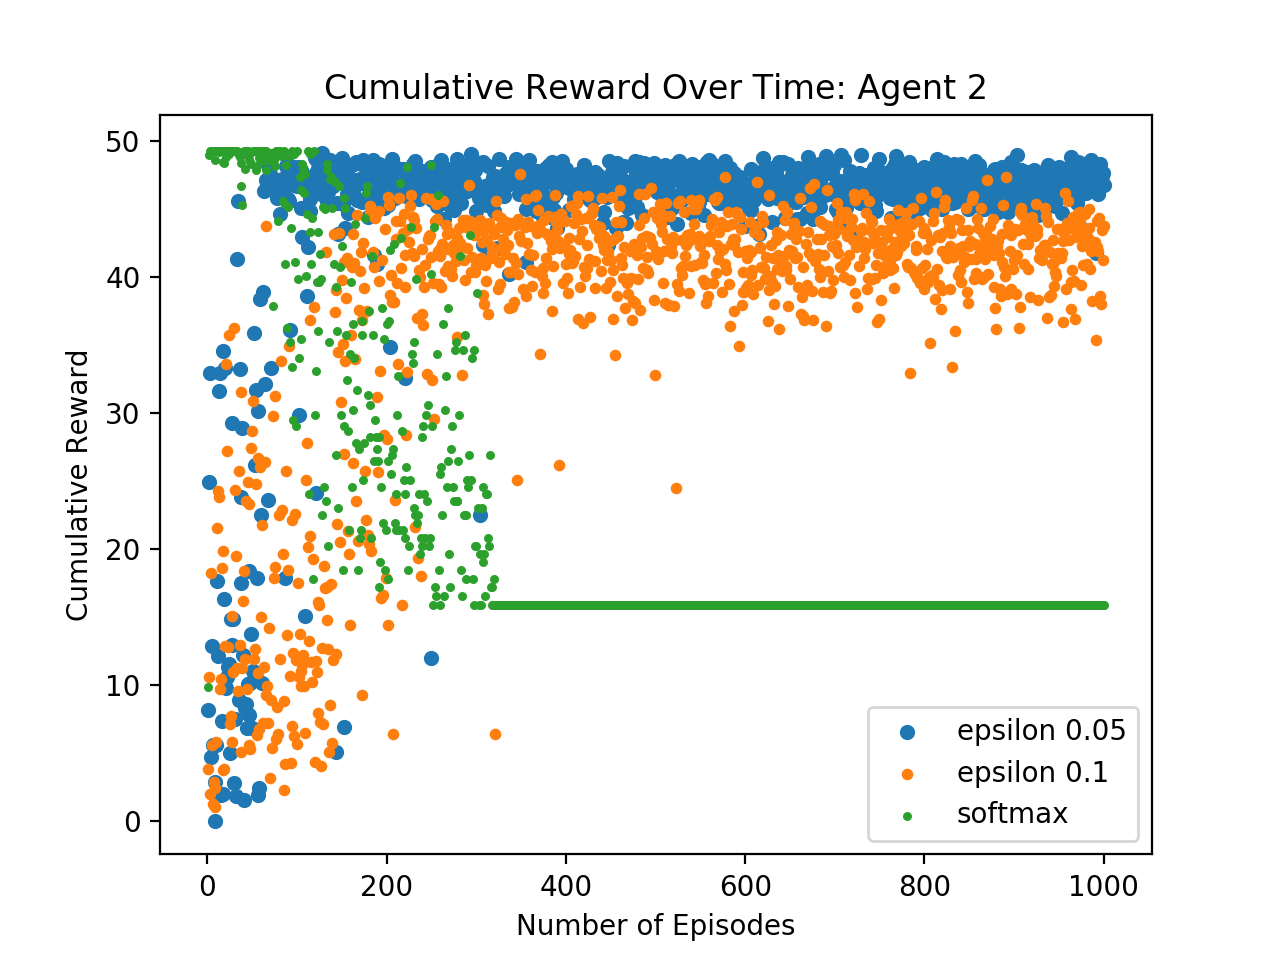
\includegraphics[width=.7\textwidth]{ai-env2-agent2}
  %\caption{Environment 2, agent 1 cumulative reward}
\end{figure}



For the epsilon algorithms, agent 2 learns pretty quickly that staying where it started is the best way of earning reward. However, the variance is quite high due to the constant exploration rate. Thankfully, for these algorithms, agent 1 never finds the closer resource, so agent 2's performance stays consistent once it learns. On the other hand, softmax learns more quickly to stay where agent 2 started. However, once agent 1 finds the resource, it becomes overcrowded and agent 2's performance significantly worsens. This triggers softmax to start exploring more often, and we have a period of high variance for agent 2 from episodes 150-350. Agent 2 quickly discovers that the farther pair does not improve the results and returns to the overcrowded resource. Agent 2 cannot do anything about the agent 1's greediness. Once softmax realizes, this, agent 2's variance decreases significantly. We now analyze the overall utility.

%[insert ai-env2.png]\\

\begin{figure}[h]
  \centering
  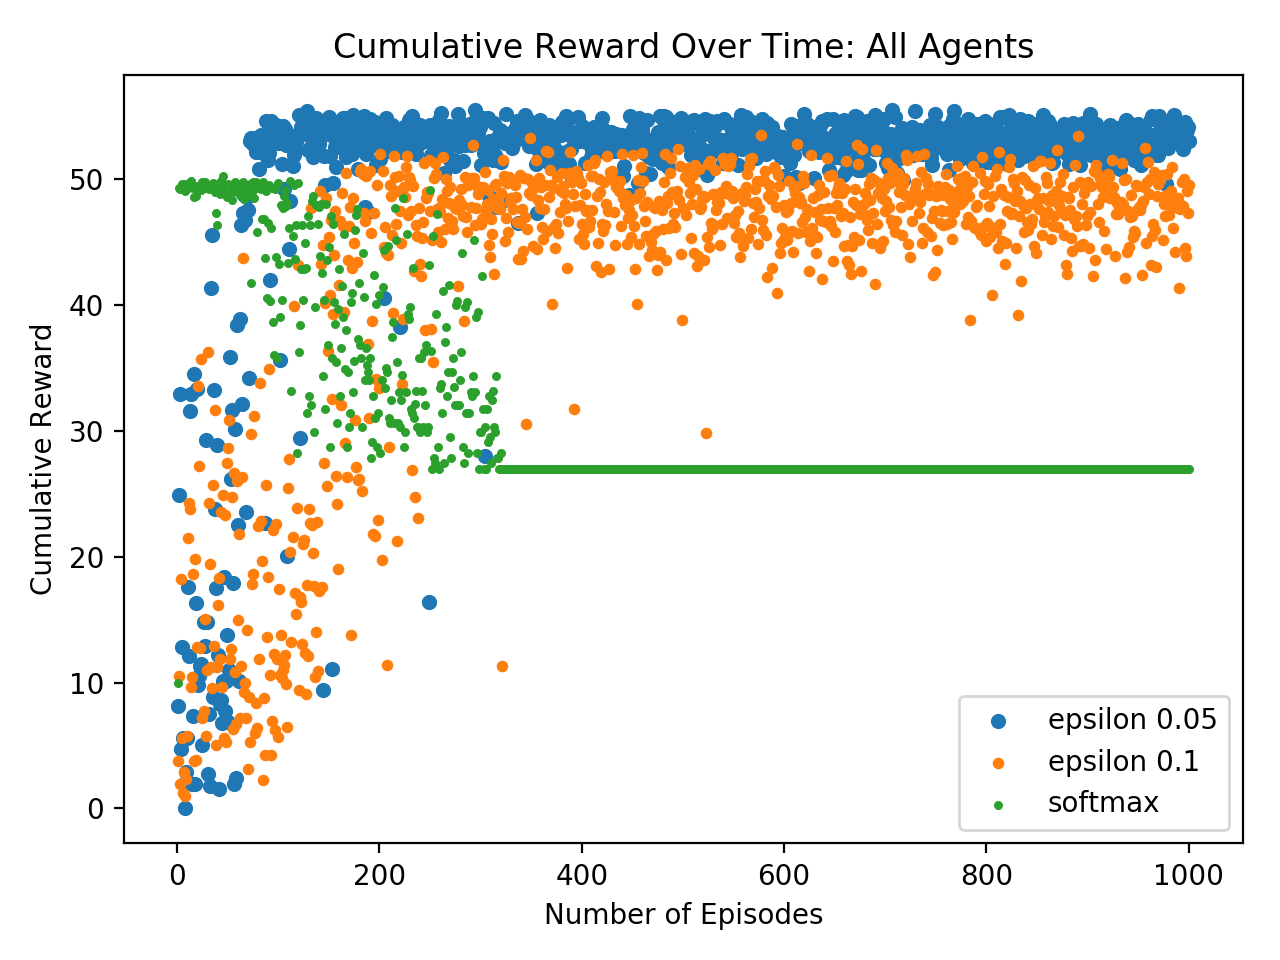
\includegraphics[width=.7\textwidth]{ai-env2}
  %\caption{Environment 2, agent 1 cumulative reward}
\end{figure}


Softmax starts out performing way better than epsilon-greedy thanks to agent 2 starting out in the perfect location. However, once agent 1 discovers the closer pair, the overall performance goes down for softmax. We notice that for the epsilon algorithms, when agent 1 never finds the location that is better for itself individually, the overall utility is better than that of softmax. This is similar to the classic prisoner's dilemma problem. We present the following game matrix with approximated values.

\begin{center}
\begin{tabular}{ c c c }
  & Far Pair & Close Pair \\ 
 Far Pair & 1, 1 & 1, 4 \\  
 Close Pair & 4, 1 & 1.5, 1.5    
\end{tabular}
\end{center}

The dominant strategy is for both agents to select the close pair, which is what happens when we use softmax for action selection. However, when one agent cannot find the close pair (when we use epsilon-greedy), overall utility is increased.

\subsection{Working Together}

We now present our results for the environment where agents have different roles. Recall that some agents are "gatherers", that is to say they can mine resources. Other agents are "carriers", and only they know the procedure for dropping them off at the spawn. All agents can carry resources around, but the gatherers must give their resources they mine to a carrier to drop off at a spawn. When we create a simple environment with only one dimension, the agents learn pretty quickly what to do. However, the agents never seem to learn for more complicated environments. We notice that at some points, the reward spikes up a bit only for it to go back down immediately.

We believe this occurs due to the fact that both agents are moving. It it is difficult for them to both be in the place they expect each other to be at the right time, and when they aren't, the q-value decreases, and they eventually find each other (randomly) somewhere else. This increases the q-value for the new meeting point, but they don't end up there at the same time again. Since the agent's don't have the other agent locations as part of their state, they see the state as the same regardless of whether or not the agents are next to each other. When the desired action is not available, the value of the state decreases due to the fact that the state takes into account the reduced future reward for it taking longer to find the other agent again.\\

\subsection{Sabotage}

In this environment, we add a thief (agent 1) who's goal is to steal resources from the other agent (agent 2). The only source only has one access point, as the others are blocked by either a blockade or an edge. The goal of the thief could theoretically make it impossible for agent 2 to stow any resources, but the thief won't get any reward unless it chases after agent 2 and steals resources. First, we present the results for the thief.

%[insert thief-agent1.png]

\begin{figure}[h]
  \centering
  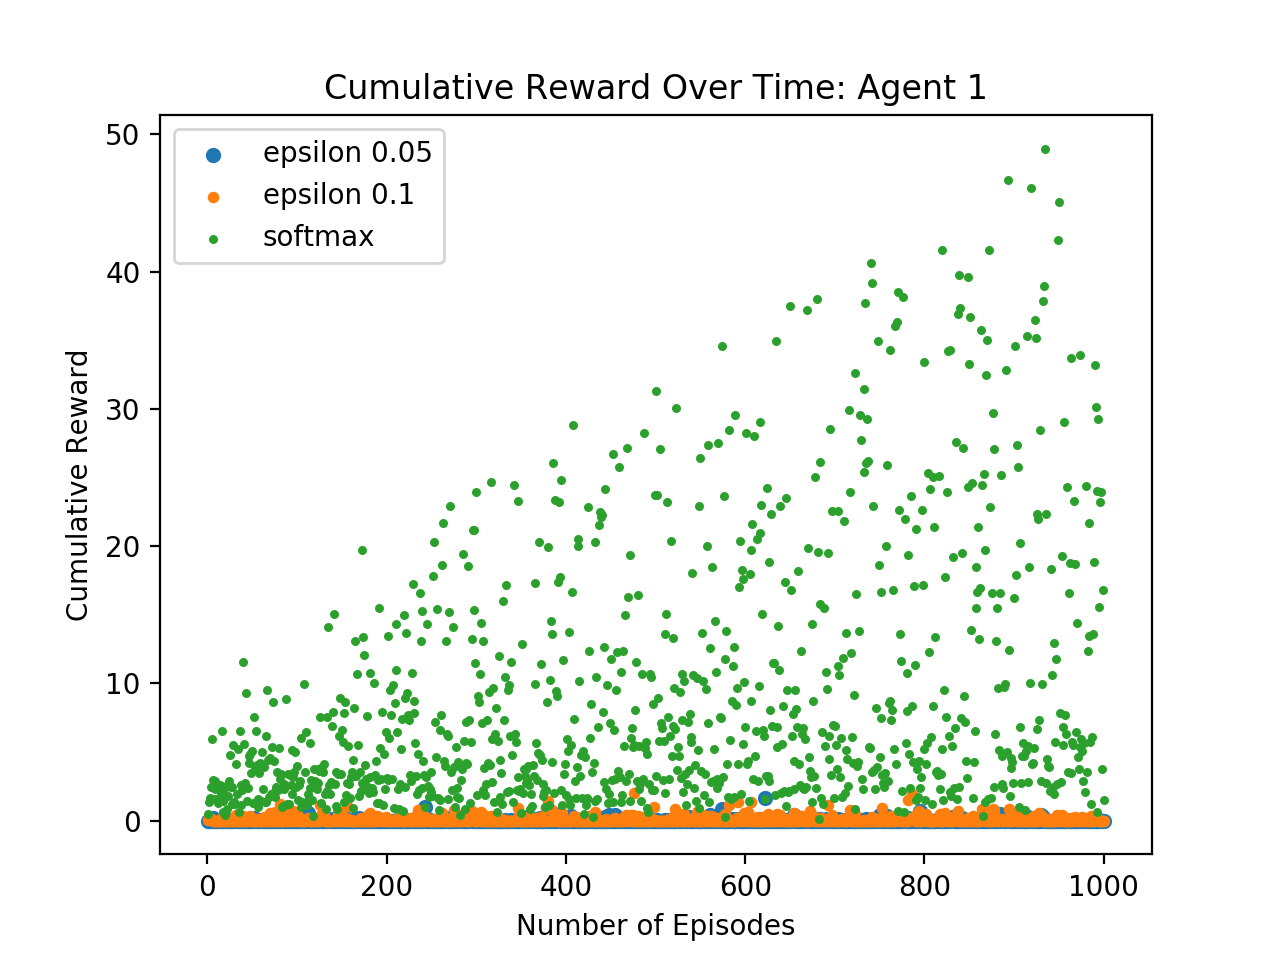
\includegraphics[width=.7\textwidth]{thief-agent1}
  %\caption{Environment 2, agent 1 cumulative reward}
\end{figure}



We notice that the thief is only successful with the softmax algorithm. Even then, the variance increases over time despite the evident learning. This is perhaps due to the unpredictable nature of the other agent. Based on our observation of the "good" agent, it alternates between running away and trying to (mostly unsuccessfully) stow a resource. We can see in the graph of agent 2 that the thief has a huge advantage here. 

%[insert thief-agent2.png]

\begin{figure}[h]
  \centering
  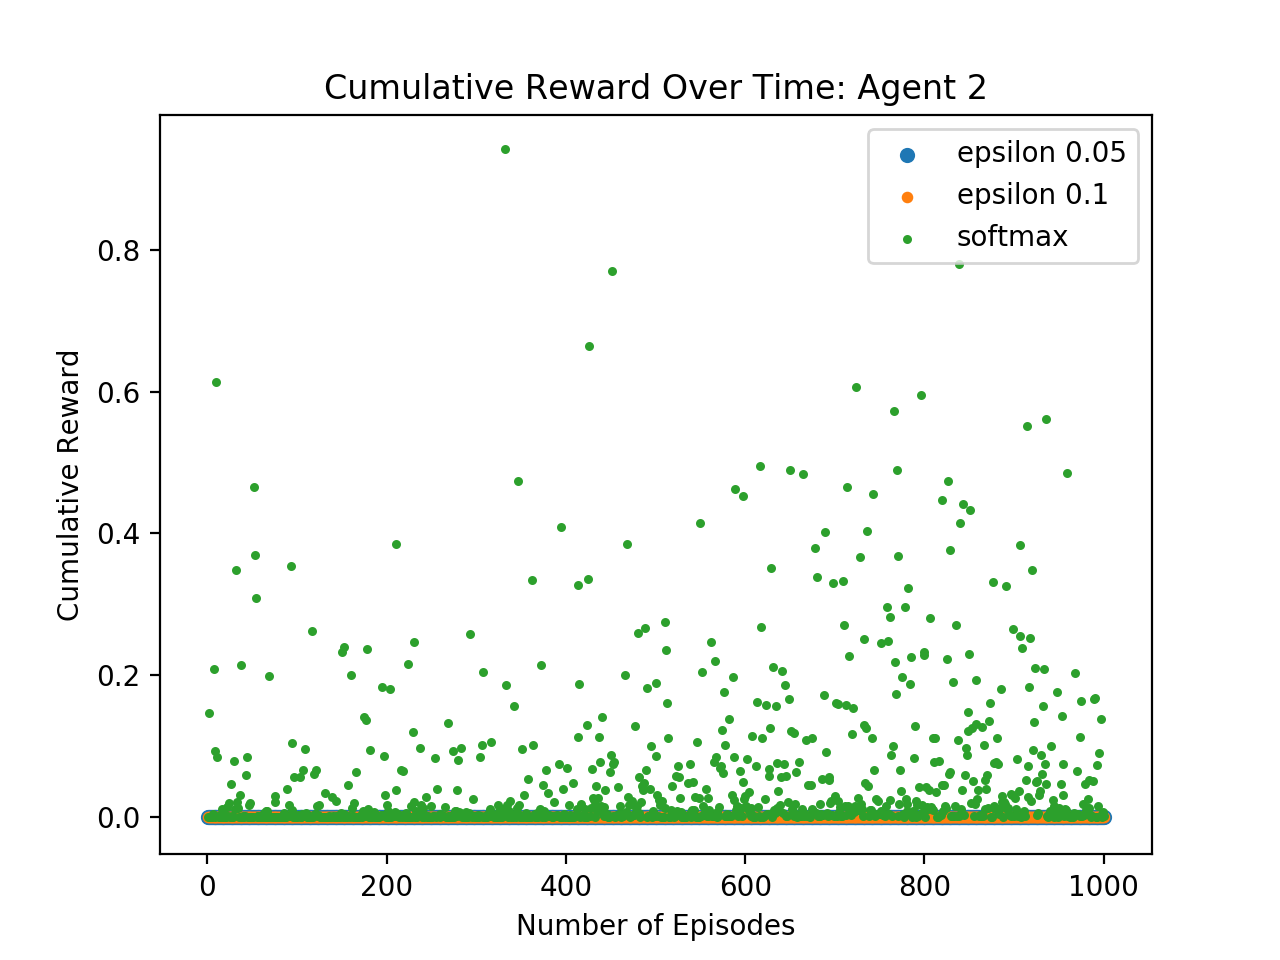
\includegraphics[width=.7\textwidth]{thief-agent2}
  %\caption{Environment 2, agent 1 cumulative reward}
\end{figure}


Ultimately what makes this environment interesting, is to think about the agent's incentives. If the thief tries chasing agent 2 around, then agent 2 might be able to run around the thief and get to the source. On the other hand, if it stays by the source, agent 2 may learn to never come near, resulting in both agents to receive minimal reward. If only the agents could agree to alternate between letting one steal and the other stow. That would cause maximum overall utility but cannot occur when they are both greedy, not to mention untrustworthy. Ultimately, the agents are making the right decision given their inability to communicate. In a larger environment, we could encounter zugzwang, a concept often used in chess to describe the situation where whoever makes the first move loses. If the thief moves away from the spawn, the agent can get there. But if the agent tries going to the spawn before the thief moves, the thief will get the agent. Whoever makes the first move loses.

\section{Future Work}

	The next step we would take in this project is to add in shared Q-tables. This would change the motivation of each agent, and instead of being greedy they would try to maximize the system's total utility. This could result in new emergent behaviors such as cooperation between thieves and their victims, where they alternate between stealing the resource and turning it in. It would also greatly increase the cooperation between gatherers and carriers, assuming we modified their states to include the location of the other.

\section{Conclusion}

	In this project, we build a simplified clone of Screeps that allowed for direct control over our experiments. We applied Q-learning techniques in a number of environments and observed the patterns of behavior that emerged. In the first environment which contained only one agent, we found that the softmax approach was able to find the most optimal solution while the epsilon-greedy approaches only found a sub-optimal solution. In the prisoners dilemma environment, we found that the system's total utility was lower when the agents favored exploration over exploitation. This is because they are greedy and non-communicating, so each will choose whichever strategy maximizes its own utility. Given the opportunity, the agent which starts far away from the optimal source-spawn path will go there even at the expense of the other. 
	
	In the environment which divides up the responsibility between gatherers and carriers, we found that cooperation is extremely hard without communication. Because each agent doesn't contain the other agent's location within its state, its Q-table fails to direct it towards the nearest potential handoff but instead towards the spot where it has most often handed off in the past. We found that when the agents met, it was usually a coincidence, indicating that little meaningful learning occurred. With the introduction of a thief agent, a whole new layer of complexity was added. Because the thief and its victim are both using Q-learning, their greedy approaches lead to a stalemate. If the thief starts camping the spawn, then its victim will learn to avoid the spawn. The behavior that emerges is "the first to move loses", where making the first move gives the other agent the advantage. This makes perfect sense in a pair of non-communicating greedy agents, because neither is willing take a negative reward by making a move that its opponent can exploit.
	
	 In the end, we created a system that allowed for the unobstructed observation of the performance of Q-learning methods in multiagent systems. Using this system, we modeled a number of different scenarios and explored the emergent behavior of non-communicating greedy agents. 

\section{References}



\end{document}

